%%
%% ****** ljmsamp.tex 13.06.2018 ******
%%
\documentclass[
11pt,%
tightenlines,%
twoside,%
onecolumn,%
nofloats,%
nobibnotes,%
nofootinbib,%
superscriptaddress,%
noshowpacs,%
centertags]%
{revtex4}
\usepackage{ljm}

\usepackage{makecell}




\begin{document}

\titlerunning{Parallel global search algorithm with local tuning} % for running heads
%\authorrunning{First-Author at al.} % for running heads
\authorrunning{Barkalov, Lebedev} % for running heads

\title{Parallel Global Search Algorithm with Local Tuning\\ 
for Solving Mixed-Integer Global Optimization Problems}
% Splitting into lines is performed by the command \\
% The title is written in accordance with the rules of capitalization.

\author{\firstname{K.~A.}~\surname{Barkalov}}
\email[E-mail: ]{konstantin.barkalov@itmm.unn.ru}
\affiliation{Lobachevsky State University of Nizhni Novgorod, Gagarin ave. 23, Nizhni Novgorod, 603950 Russia}


\author{\firstname{I.~G.}~\surname{Lebedev}}
\email[E-mail: ]{ilya.lebedev@itmm.unn.ru}
\affiliation{Lobachevsky State University of Nizhni Novgorod, Gagarin ave. 23, Nizhni Novgorod, 603950 Russia}
%\noaffiliation % If the author does not specify a place of work.

\firstcollaboration{(Submitted by A.~A.~Editor-name)} % Add if you know submitter.
%\lastcollaboration{ }

\received{February 1, 2021} % The date of receipt to the editor, i.e. December 06, 2017


\begin{abstract} % You shouldn't use formulas and citations in the abstract.
В работе рассматриваются mixed-integer global optimization problems. Обсуждается параллельный алгоритм для решения задач данного класса, основанный на information-statistical approach к решению задач непрерывной глобальной оптимизации. Для рассматриваемого параллельного алгоритма предложена схема локальной настройки, основанная на предположении слабой многоэкстремальности задачи. 
Приведены результаты сравнения последовательной версии алгоритма с другими методами аналогичного назначения. 
Эффективность распараллеливания алгоритма подтверждена решением серии mixed-integer global optimization problems на Lobachevsky supercomputer. 
\end{abstract}

\subclass{90C26, 90C30} % Enter 2010 Mathematics Subject Classification.

\keywords{Global optimization, Non-convex constraints, Mixed-integer problems, Local tuning, Parallel algorithms} % Include keywords separeted by comma.

\maketitle

% Text of article starts here.

\section{Introduction}

В работе рассматриваются global optimization problems и параллельные методы их решения. Методы решения задач указанного класса  обладают значительной вычислительной трудоемкостью, т.к. глобальный оптимум является интегральной характеристикой решаемой задачи и требует исследования всей области поиска. Как результат, поиск глобального оптимума сводится к построению некоторого покрытия (как правило, неравномерного) в области изменения параметров. Особый интерес представляют задачи, в которых часть параметров может принимать лишь дискретные (например, целочисленные) значения (mixed-integer global optimization problems), т.к. для них сложнее построить оценки оптимума по сравнению с задачами, в которых все параметры являются непрерывными.

Ситуация, когда некоторые из параметров характеризуются дискретностью, является широко распространенной в прикладных оптимизационных задачах. При этом дискретные параметры имеют, как правило, небольшое число значений и могут определять, например, марку используемого материала, вариант типовой компоновки деталей и т.п. 
Одновременно с этим целевая функция и ограничения обычно заданы не явно, а в виде некоторого алгоритма вычисления их значений в точках области поиска, т.е. представляют собой функции вида “black-box”. Процесс проверки ограничений и вычисления значения целевой функции в некоторой точке (называемый в дальнейшем trial) требует проведения численного моделирования и является трудоемкой операцией. 

Методам решения mixed-integer problems посвящена обширная литература (см., например, обзоры \cite{Burer,Boukouvala}). Известные детерминированные методы решения задач данного класса основаны, как правило, на подходах Branch-and-Bound \cite{Belotti} or Branch-and-Reduce \cite{Vigerske}. Для решения таких задач могут применяться также nature-inspired algorithms \cite{Deep,Schluter}, которые так или иначе основаны на идеях случайного поиска.

Отметим ключевые моменты, специфичные для построения параллельных алгоритмов решения mixed-integer global optimization problems. Организовать распараллеливание процесса поиска можно несколькими способами.
Во-первых, можно распараллеливать процесс проведения одного trial, т.е. вычисления функций задачи в одной точке области поиска. Данный путь будет давать ускорение, но является специфичным для каждой конкретной решаемой задачи.
Во-вторых, можно распараллелить реализацию вычислительных правил алгоритма, обеспечивающих выбор точки очередного испытания. В этом случае способ распараллеливания будет зависеть от конкретного класса алгоритмов и, кроме того, часто эти правила достаточно просты и распараллеливать их нецелесообразно.
В-третьих, можно организовать параллельное выполнение нескольких испытаний на одной итерации поиска. Этот подход и будет использоваться в данной работе, т.к. он характеризуется эффективностью (распараллеливается именно та часть вычислительного процесса, в которой выполняется основной объем вычислений) и общностью (применим для широкого класса алгоритмов глобальной оптимизации).

В данной работе нами предложен новый параллельный метод решения mixed-integer problems, основанный на information-statistical approach к решению задач глобальной оптимизации \cite{Strongin2000,Strongin2013}. 

В рамках данного подхода 
\begin{itemize}
	\item 
	решение многомерных задач сводится  к решению эквивалентных им одномерных, cоответствующая редукция основана на использовании space-filling curves;
	\item 
	при решении constrained optimization problems каждое ограничение учитывается и обрабатывается отдельно, штрафные функции не используются;
	\item
	учитывается информация о неоднородном поведении функций задачи в разных подобластях областях области поиска, что позволяет ускорить процесс поиска решения за счет совмещения процедур локального уточнения текущего лучшего решения и его глобального обновления;
	\item 
	распараллеливание процесса поиска осуществляется за счет одновременного вычисления на каждой итерации нескольких значений целевой функции в разных точках search domain.	
\end{itemize}

Текст статьи, отражающей результаты проведенного исследования, построен следующим образом. 
В Section 2 дано краткое описание описание схемы редукции размерности с использованием space-filling curves, а также описана индексная схема учета ограничений. Здесь же приведена формулировка параллельного индексного алгоритма для решения задач непрерывной глобальной оптимизации.
В Section 3 изложен способ учета локальных свойств функций задачи, позволяющий ускорить сходимость алгоритма.
В Section 4 предложен подход к обобщению параллельного индексного алгоритма с целью решения mixed-integer problems. Приведен способ, позволяющий свести решение mixed-integer problem к решению информационно-связанного множества задач непрерывной оптимизации, которое может выполняться параллельно. 
Section 5 содержит результаты численных экспериментов. Здесь производится сравнение последовательной версии алгоритма с известными аналогами, а также показана эффективность распараллеливания алгоритма с локальной настройкой при решении серии multiextremal mixed-integer problem на суперкомпьютере.  
Section 6 concludes the paper.

\section{Parallel global optimization algorithm and dimensionality reduction}

Рассмотрим задачу глобальной оптимизации с непрерывными параметрами вида
\begin{eqnarray}\label{problem}
&\varphi(y^\ast)=\min{\left\{\varphi(y):y\in D, \; g_i(y)\leq 0, \; 1 \leq i \leq m\right\}},\\
&D=\left\{y\in R^N: a_j\leq y_j \leq b_j, 1\leq j \leq N \right\}.\label{D}
\end{eqnarray}
Будем предполагать, что objective function $\varphi(y)$ (hereafter denoted by $g_{m+1}(y)$) and the left-hand sides $g_i(y), \; 1\leq i \leq m,$ of the constraints satisfy the Lipschitz condition 
\[
\left|g_i(y_1)-g_i(y_2)\right|\leq L_i\left\|y_1-y_2\right\|, \;1\leq i\leq m+1, \; y_1,y_2 \in D,\;
\]
with a priori unknown constants $L_i, \; 1 \leq i \leq m+1$. 

Предположение о выполнении условия Липшица является типичным для многих подходов к построению параллельных алгоритмов глобальной оптмизации \cite{Evtushenko2009,Zilinskas2011}. При этом для решения многомерных задач оптимизации адаптируются алгоритмы решения одномерных задач, см., например, методы на основе разбиений области поиска \cite{Zilinskas2014,Sergeyev2017}.

В данной работе мы будем использовать подход к сведению многомерных задач к одномерным на основе space-filling curves. 
Используя отображения типа Peano-Hilbert curve $y(x)$, отображающие отрезок $[0,1]$ на $N$-dimensional domain (\ref{D}),
можно свести многомерную задачу условной минимизации в области $D$ к одномерной задаче условной минимизации на отрезке $[0,1]$
\begin{equation}\label{problem1}
\varphi(y(x^\ast))=\min \left\{\varphi(y(x)): x \in [0,1], \; g_i(y(x))\leq 0, \; 1 \leq i \leq m\right\}.
\end{equation}

Методы для построения чиcленных аппроксимаций Peano-Hilbert curve $y(x)$ (называемых \textit{evolvent}) рассмотрены в \cite{Sergeyev2013}. These evolvents are fractals generated by an iterative process, that fill in the hypercube $D$ with accuracy $2^{-M}$, where integer $M>0$ is the evolvent construction parameter. 
Примеры разверток с разными значениями $M$  для размерности $N=3$ приведены на Fig.~\ref{evolvents}.

\begin{figure}
\begin{minipage}{0.4\linewidth}
\center{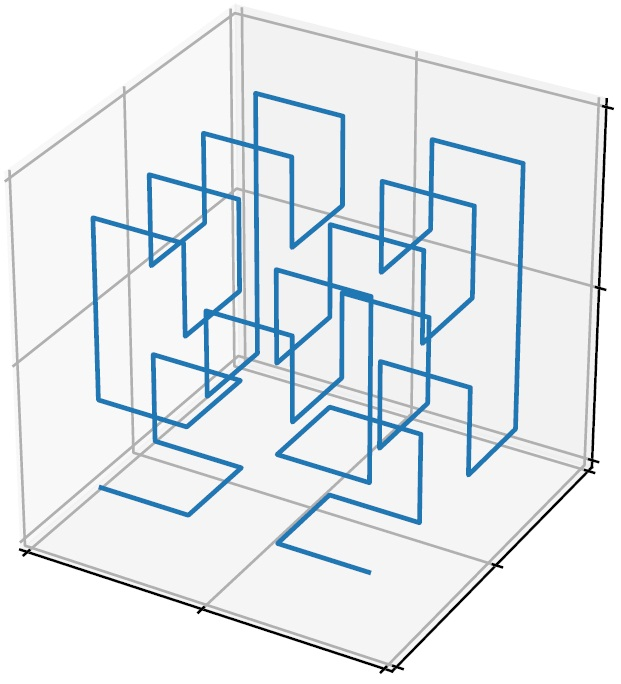
\includegraphics[width=1.0\linewidth]{fig1b.JPG} \\ (a)}
\end{minipage}
\begin{minipage}{0.4\linewidth}
\center{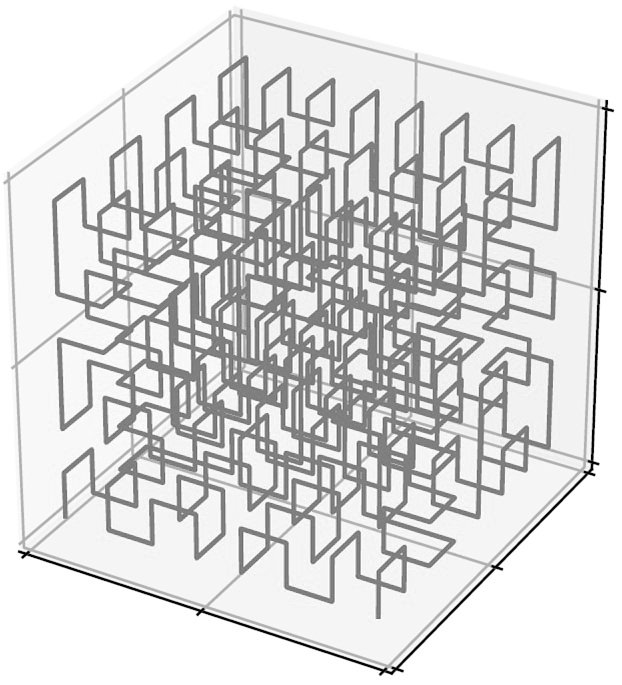
\includegraphics[width=1.0\linewidth]{fig1c.JPG} \\ (b)}
\end{minipage}
\caption{Evolvents in three dimensions with (a) $M=3$ and (b) $M=4$}
\label{evolvents}
\end{figure}

Задачу (\ref{problem1}) мы будем рассматривать в предположении, что функции $g_i(y(x))$ определены и вычислимы лишь на соответствующих множествах 
\[
Q_1=[0,1], \; Q_{i+1}=\left\{x \in Q_i : g_i(y(x)) \leq 0 \right\}, \; 1 \leq i \leq m.
\]

Эти условия позволяют ввести классификацию точек $x \in [0,1]$ в соответствии с числом $\nu (x)$ ограничений, вычисленных в этой точке. The \textit{index} $\nu(x)$ также можно определить с помощью условий
\begin{equation}\label{nu}
g_i(y(x)) \leq 0, \; 1 \leq i < \nu, \; g_\nu(y(x))>0,
\end{equation}
где последнее неравенство исключается из рассмотрения, если $\nu=m+1$.

Указанная схема редукции размерности сопоставляет многомерной задаче с липшицевой минимизируемой функцией и липшицевыми ограничениями одномерную задачу, в которой соответствующие функции удовлетворяют uniform H{\"o}lder condition (see \cite{Sergeyev2013}), i.e.,
\[
\left|g_i(y(x_1))-g_i (y(x_2))\right| \leq H_i \left|x_1-x_2 \right|^{1/N}, \; x_1,x_2\in [0,1], \; 
1\leq i \leq m+1,
\]
где $N$ есть размерность исходной многомерной задачи, а H{\"o}lder coefficients $H_i$ связаны с Lipschitz constants $L_i$ исходной задачи соотношениями $H_i \leq 2L_i \sqrt{N+3}$.

Таким образом, \textit{a trial} в точке $x^k \in [0,1]$, выполненное на $k$-й итерации алгоритма, будет состоять из следующих действий:
\begin{itemize}
	\item определить \textit{image} $y^k=y(x^k)$ в соотвествии с отображением $y(x)$;
	\item вычислить значения $g_1(y^k),..., g_\nu(y^k),$ where $\nu = \nu(x^k)$ is from (\ref{nu}). 
\end{itemize}
Пару значений 
\begin{equation} \label{trial_result}
 \{ \nu=\nu(x^k), \; z^k=g_\nu(y(x^k)) \} 
\end{equation}
порождаемую испытанием в точке $x^k \in [0,1]$, будем называть \textit{trial outcome}.

Рассмотрим параллельный алгоритм для решения constrained global optimization problems, предложенный в работах \cite{Strongin2000,Strongin2013} и основанный на индексной схеме учета ограничений. 

При описании параллельного алгоритма мы будем предполагать, что в нашем распоряжении имеется $p$ вычислительных элементов (узлов, процессоров или ядер), которые будут использоваться для параллельного проведения $p$ trials одновременно. 

На первой итерации метода $p$ trials проводятся параллельно в произвольных различных точках $x^i\in(0,1)$, $1\leq i \leq p$.
Пусть выполнено $n\geq 1$  итераций метода, в процессе которых были проведены испытания в $k=np$ точках $x^i, 1\leq i \leq k$. Тогда точки $x^{k+1},...,x^{k+p}$ поисковых испытаний $(n+1)$-ой итерации определяются в соответствии со следующими правилами.

\begin{enumerate}
\item 
Перенумеровать точки $x^1,...,x^k$ предшествующих испытаний нижними индексами в порядке увеличения значений координаты
\begin{equation}\label{Eq:17}
0=x_0<x_1<...<x_i<...<x_k<x_{k+1}=1,
\end{equation}
и сопоставить им значения $z_i=g_\nu(y(x_i))$, $\nu=\nu(x_i)$, $1 \leq i \leq k$, из (\ref{trial_result}), вычисленные в этих точках; точки $x_0=0$ and $x_{k+1}=1$ введены дополнительно; значения $z_0$ и $z_{k+1}$ не заданы.
\item
Провести классификацию номеров  $i,1\leq i \leq k$, точек испытаний из  (\ref{Eq:17}) по числу ограничений задачи, выполняющихся в этих точках, путем построения множеств
\begin{equation}\label{Eq:18}
I_\nu = \left\{i: 1 \leq i \leq k,\ \nu = \nu(x_i)\right\},\ 1 \leq \nu \leq m+1,
\end{equation}
содержащих номера всех точек  $x_i,1\leq i \leq k$, имеющих индексы, равные одному и тому же значению $\nu$. Граничные точки $x_0=0$ and $x_{k+1}=1$ интерпретируются как имеющие нулевые индексы, и им сопоставляется дополнительное множество $I_0={0,k+1}$. 

Определить максимальное значение индекса
\begin{equation}\label{Eq:19}
V=\max \left\{\nu = \nu(x_i), \ 1\leq i \leq k\right\}.
\end{equation}
\item
For all values of $\nu, \ 1\leq \nu \leq m+1$, calculate the values  
\begin{equation}\label{Eq:20}
\mu_\nu = \max \left\{ \frac{\left|z_i-z_j\right|}{\left(x_i-x_j\right)^{1/N}} : i,j \in I_\nu, j<i\right\}.
\end{equation}
Если множество  $I_\nu$ содержит менее двух элементов или если $\mu_\nu$ from (\ref{Eq:20}) оказывается равным нулю, то использовать значение $\mu_\nu=1$.
\item
Для всех непустых множеств  $I_\nu$, $1 \leq \nu \leq m+1$, вычислить значения
\begin{equation}\label{Eq:21}
  z^\ast_\nu =  
   \begin{cases}
    -\epsilon_\nu,  \nu < V, \\
    \min{\left\{g_\nu(x_i):i\in I_\nu\right\}}, \nu = V,
   \end{cases}
\end{equation}
где $V$ является максимальным значением индекса, а вектор
\begin{equation}\label{Eq:22}
\epsilon _R=\left(\epsilon_1,...,\epsilon_m\right),
\end{equation}
с положительными компонентами (называемый также \textit{reserve vector}) является параметром алгоритма.
\item
Для каждого интервала  $(x_{i-1},x_i)$,$1 \leq i \leq k+1$, вычислить \textit{характеристику} $R(i)$: 
\begin{eqnarray}\label{R}
&R(i)=\Delta_i+ \frac{(z_i-z_{i-1})^2}{(r_\nu\mu_\nu)^2\Delta_i}-2\frac{z_i+z_{i-1}-2z^\ast_\nu}{r_\nu\mu_\nu},\;\; \nu=\nu(x_{i-1})=\nu(x_i),\nonumber \\
&R(i)= 2\Delta_i-4\frac{z_i-z^\ast_\nu}{r_\nu\mu_\nu},\;\; \nu(x_{i-1})<\nu(x_i)=\nu,\\
&R(i)= 2\Delta_i-4\frac{z_{i-1}-z^\ast_\nu}{r_\nu\mu_\nu},\;\; \nu = \nu(x_{i-1})>\nu(x_i).\nonumber
\end{eqnarray}
где $\Delta_i=(x_i-x_{i-1})^{1/N}$, а значения $r_\nu>1, 1\leq\nu\leq m+1$, являются параметрами алгоритма.
\item
Упорядочить характеристики $R(i)$, $1\leq i \leq k+1$, по убыванию  	
\begin{equation}\label{Eq:23}
R(t_1)\geq R(t_2)\geq ... \geq R(t_{k})\geq R(t_{k+1})
\end{equation}
и выбрать $p$ интервалов с номерами $t_j, 1\leq j \leq p$, которым соответствуют наибольшие характеристики.
\item
Провести параллельно $p$ новых испытаний в точках $x^{k+j}, 1 \leq j \leq p$, вычисленных по формулам
\begin{eqnarray*}
& x^{k+j}=\frac{x_{t_j}+x_{t_j-1}}{2}, \; \nu(x_{t_j-1})\neq \nu(x_{t_j}), \\
& x^{k+j}=\frac{x_{t_j}+x_{t_j-1}}{2}- \frac{\mathrm{sign}(z_{t_j}-z_{t_j-1})}{2r_\nu}\left[\frac{\left|z_{t_j}-z_{t_j-1}\right|}{\mu_\nu}\right]^N, \; \nu(x_{t_j-1})=\nu(x_{t_j})=\nu. \\
\end{eqnarray*} 

\end{enumerate}

Алгоритм прекращает работу, если по крайней мере для одного из номеров $t_j, 1\leq j \leq p$ выполняется условие $\Delta_{t_j}\leq \epsilon$; здесь $\epsilon>0$ есть заданная точность решения задачи.

Данный способ организации параллельных вычислений имеет следующее обоснование. Используемые в вычислительных правилах алгоритма характеристики интервалов (\ref{R}) могут рассматриваться как некоторые оценки вероятности обнаружения в данных интервалах точки глобального минимума. Неравенства (\ref{Eq:23}) упорядочивают интервалы по их характеристикам, и испытания проводятся параллельно в первых $p$ интервалах, имеющих наибольшие вероятности.

A detailed description of the algorithm convergence theory is presented in \cite{Strongin2000,Strongin2013}.
Роль параметров алгоритма ($r_\nu>1$ and $\epsilon_\nu>0, 1\leq\nu\leq m+1$) обсуждается в \cite{Strongin2020}.
Изложенный алгоритм может быть также использован для решения задач многокритериальной оптимизации \cite{Gergel2020}.

\section{Local tuning for global optimization algorithm}

Одно из важных свойств рассматривамых задач заключается в том, что во многих случаях поведение функций в задаче многоэкстремальной оптимизации является неоднородным в разных подобластях поиска. В некоторых подобластях значения функций могут изменяться достаточно быстро (что будет соответствовать большим значениям константы Липшица в таких подобластях), в других подобластях значения могут изменяться более плавно. Как результат, построение единых оценок характеристик функции для всей области поиска может не полностью соответствовать ее поведению в конкретной подобласти. 

Детально проработанным направлением здесь является использование разных оценок константы Липшица для каждого поискового интервала в отдельности \cite{Sergeyev2003,Sergeyev2007}. Определенная сложность здесь состоит в том, что при построении локальных оценок константы Липшица неявно предполагается квадратичное поведение функции в малой окрестности исследуемой точки, что может негативно сказаться на работе метода вне этой окрестности. 
Одновременно с этим при вычислении локальных (интервальных) оценок должна учитываться и общая (глобальная) оценка константы Липшица, что приводит к использованию сложных компромиссных схем оценивания константы \cite{Sergeyev2020}.

Более удобным подходом, учитывающим неоднородность поведения функций задачи в разных подобластях области поиска,  является адаптивное прогнозирование положения оптимума на основе накопленной поисковой информации в предположении слабой многоэкстремальности задачи. Основы подхода изложены в \cite{Strongin2000}, некоторые результаты решения задач на параллельных вычислительных системах приведены в \cite{Barkalov2010}.

В соответствии с данным подходом можно построить адаптивные правила прогнозирования, основанные на предположении о том, что местонахождение глобального оптимума более вероятно в окрестностях тех точек из ряда $x_i, 1 \leq i \leq k,$ которым соответствуют малые значения нормированных разностей $\omega_i=(z_i-z_\nu^*)/\mu_\nu$, где $\mu_\nu$ из (\ref{Eq:20}), а $z_\nu^*$ из (\ref{Eq:21}).

Принятая гипотеза правдоподобна либо в случае, когда число осуществленных итераций достаточно велико (т.к. алгоритм при выполнении условий сходимости порождает последовательность испытаний, плотную лишь в точках глобального минимума), либо в случае, когда задача является унимодальной (т.е. когда поиск в окрестности лучшего текущего приближения позволяет достичь улучшения, и такие последовательные улучшения ведут к решению). Первый случай соответствует заключительной фазе поиска, и тогда использование адаптивного прогноза можно интерпретировать как способ ускорения уточнения решения. Второй случай фактически включает в себя предположения о слабой многоэкстремальности задачи.

Новые формулы для вычисления характеристик поисковых интервалов $R'(i)$, которые должны быть использованы на 5-м шаге алгоритма, могут быть представлены в виде 
\[
R'(i) = h_i R(i),
\]
где $R(i)$ из (\ref{R}), а множитель $h_i$ вычисляется по правилам
\begin{eqnarray}\label{lR}
& h_i = \left[\frac{\sqrt{(z_i-z_\nu^*)(z_{i-1}-z_\nu^*)}}{\mu_\nu}+10^{-q}\right]^{-1}, \; \nu(x_{i-1})=\nu(x_{i}),\nonumber\\
& h_i = \left[\frac{z_i-z_\nu^*}{\mu_\nu}+10^{-q}\right]^{-1}, \; \nu(x_{i-1})<\nu(x_{i}),\\
& h_i = \left[\frac{z_{i-1}-z_\nu^*}{\mu_\nu}+10^{-q}\right]^{-1}, \; \nu(x_{i-1})>\nu(x_{i}).\nonumber
\end{eqnarray}
Здесь целочисленный неотрицательный параметр $q$ характеризует «степень локальности» поиска: при $q=0$ поиск будет иметь ``глобальный'', а при $q>1$ -- ``локальный'' характер. 
В самом деле, множитель $h_i$ будет принимать наибольшее значение равное $1.5^q$ лишь для тех интервалов, граничные точки которых соответствуют текущему минимуму, т.е. для которых выполняется равенство $\omega_i = 0$. Указанное значение множителя $h_i$ будет большим при больших значениях параметра $q$ (что увеличит значение характеристики данного интервала), и будет равно 1 при $q=0$ (что соответствует исходному значению характеристики). 

Управление параметром $q$, входящим в (\ref{lR}), позволяет учитывать различные предположения о характере экстремума. Например, одной из стратегий управления является чередование с заданной частотой больших и малых значений $q$, что соответствует смеси локального и глобального поиска, которую можно интерпретировать как сочетание процедуры локального уточнения текущего решения и процедуры глобального обновления этого решения. При этом в течение первых итераций рекомендуется использовать значение $q=0$, т.к. накопленная на них поисковая информация обеспечит адекватность формул (\ref{lR}) при последующем локальном уточнении.


\section{Parallel algorithm for mixed-integer problems}

Рассмотрим теперь случай, когда аргумент функций задачи содержит две компоненты: вектор $y$, принадлежащий гиперинтервалу $D$, и вектор $u$, имеющий конечный (и при этом не очень большой) набор возможных значений, т.е. 
\begin{eqnarray}\label{problem_i}
& \min{\left\{ g_{m+1}(y,u):y\in D, \; g_i(y,u)\leq 0, \; 1 \leq i \leq m\right\}},\\
& D=\left\{a_j\leq y_j \leq b_j, \; 1\leq j \leq N \right\}.\nonumber
\end{eqnarray}

Такие конечные наборы могут характеризовать, например, вариант материала, из которого создается объект, геометрические размеры или другие величины, которые могут принадлежать стандартному дискретному множеству, и т.п.

Занумеруем целыми числами $s, 1\leq s \leq S,$ все возможные значения вектора $u$, т.е. сопоставим каждому рассматриваемому значению $s$ вектор $u_s$. 
Тогда рассматриваемая задача может быть записана в виде 
\begin{eqnarray}\label{problem_is}
& \min_{s\in\{1,...,S\}}\left(\min{\left\{ g_{m+1}(y,u_s):y\in D, \; g_i(y,u_s)\leq 0, \; 1 \leq i \leq m\right\}}\right),\\
& D=\left\{ a_j\leq y_j \leq b_j, \; 1 \leq j\leq N \right\}.\nonumber 
\end{eqnarray}

Используя схему редукции размерности с помощью Hilbert curve $y(x), x\in [0,1]$ можно сопоставить каждой задаче минимизации по $y$ одномерную задачу минимизации
\[
 \min{\left\{ g_{m+1}(y(x),u_s):x \in [0,1], \; g_i(y(x),u_s)\leq 0, \; 1 \leq i \leq m\right\}}, s\in\{1,...,S\}.
\]

Рассмотрим теперь отображение 
\[
Y(x)=y(x-E(x)), \; x\in[0,S],
\]
ставящее в соответствие точке из интервала [0,S] точку в области $D$ (обозначение $E(x)$ соответствует целой части числа $x$) и определим функции 
\[
f_i(x) = g_i(Y(x),u_{E(x)+1}), x\in[0,S],
\]
имеющие, вообще говоря, разрывы первого рода в целочисленных точках $x_k = i, 1\leq i \leq S-1$.
Значение  $z_k = g_\nu(y(x_k))$ из (\ref{trial_result}) в этих точках будем считать неопределенным, а значения индекса -- равным 0, т.е. $\nu(x_k) = 0$ .

Используя введенные обозначения можно переформулировать исходную задачу как
\begin{equation}\label{problem_is1}
\min \left\{f_{m+1}(x): x \in [0,S], \; f_i(x) \leq 0, \; 1 \leq i \leq m\right\}.
\end{equation}

Для иллюстрации на Fig. \ref{fig:1}  изображены графики функций, соответствующих задаче с одним непрерывным и одним бинарным параметром.
\begin{figure}[ht]
    \centering
    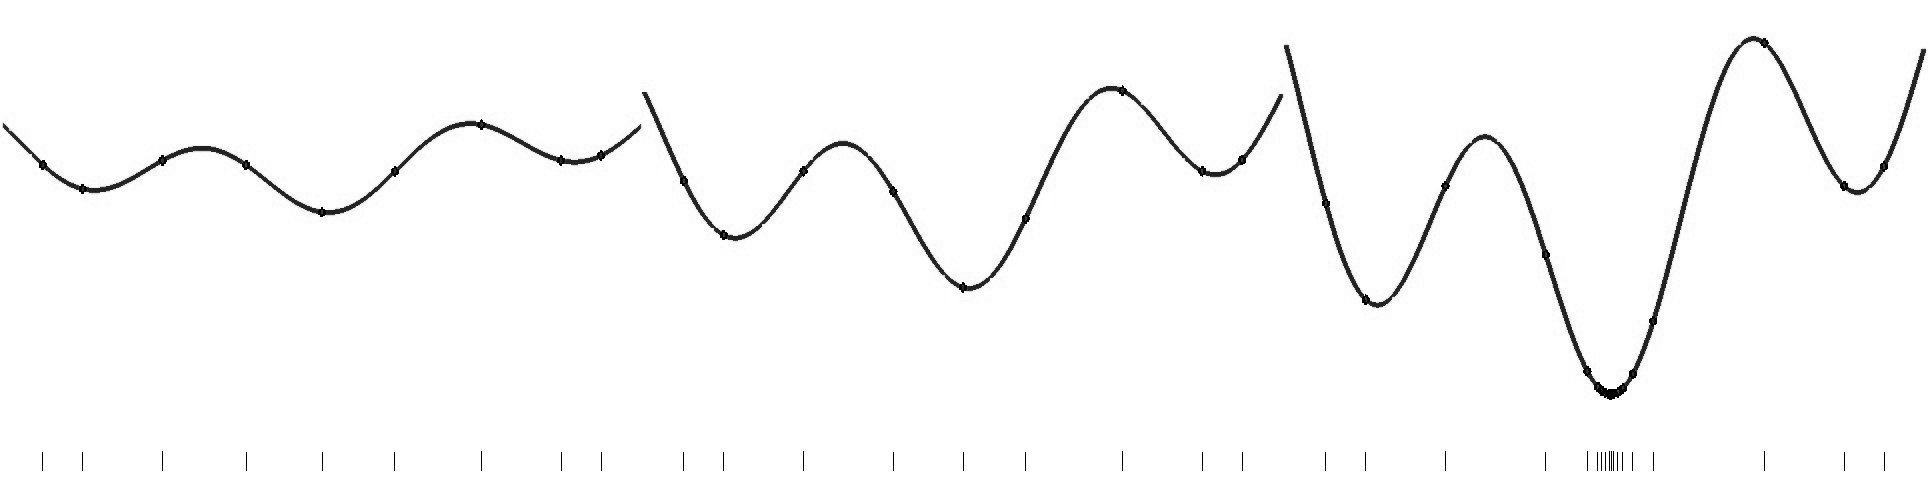
\includegraphics[width=0.7\textwidth]{fig1.jpg}
    \caption{Mixed-integer global optimization problem}
    \label{fig:1}
\end{figure}

Применяя к решению задачи (\ref{problem_is1}) параллельный индексный алгоритм с локальной настройкой, мы найдем решение задачи (\ref{problem_i}). При этом основная часть испытаний будет проведена в той подзадаче, решение которой соответствует решению исходной задачи (\ref{problem_i}). В остальных подзадачах будет проведена лишь незначительная часть испытаний, т.к. решения данных подзадач являются локально-оптимальными по отношению к решению $s$-й подзадачи. Сказанное подтверждается Fig. \ref{fig:1}, где штрихами обозначены точки испытаний, выполненных при решении данной задачи.

Таким образом, мы сформировали Parallel Mixed-integer Global search Algorithm with Local tuning (PMGAL), основанный на сведении задачи mixed-integer non-convex optimization problem к одновременно решаемому набору непрерывных задач.

Предложенная схема решения mixed-integer global optimization problems основана на параллельном индексном методе для решения задач непрерывной оптимизации и не является ориентированной на конкретное вычислительное устройство. Одной из ключевых операций здесь является параллельное проведение нескольких испытаний в различных точках области поиска (см. шаг 7 алгоритма), которое может быть реализовано как на CPU (с использованием OpenMP и/или MPI), так и на GPU (с использованием CUDA). 
В данной работе для распараллеливания были задействованы только центральные процессоры. Распределение работ между узлами осуществлялось в соответствии с многоуровневой схемой декомпозиции параллельных вычислений, изложенной в \cite{Strongin2018,Barkalov2020}.

\section{Results of experiments}

%Переводить до конца, т.е. до acknowledgments

Первая серия экспериментов была проведена с использованием последовательной версии алгоритма без использования local tuning с целью его сравнения с известными методами аналогичного назначения.

Предложенный в данной работе алгоритм PMGAL (в его последовательном варианте) сравнивался с genetic algorithm for solving mixed-integer optimization problems, реализованным в Matlab Global Optimization Toolbox. В Table \ref{tab:1} приведено число trials, потребовавшееся для решения данными методами ряда тестовых mixed-integer problems, взятых из \cite{Deep,Floudas}. Для обоих методов была использована одинаковая точность поиска решения $10^{-2}$. Все вычислительные эксперименты были проведены на компьютере с процессором Intel Core i5-7300 2.5 GHz и 8 Gb RAM. Результаты экспериментов показывают превосходство метода PMGAL как по числу итераций, так и по времени работы.

\begin{table}
	\caption{Сравнение эффективности методов PMGAL и GA}
	\label{tab:1}
	\center
	\begin{tabular}{|c|c|c|c|c|}
		\hline
	\multirow{2}{*}{Test problem}	 & \multicolumn{2}{c|}{ GA } &  \multicolumn{2}{c|}{MIGSA} \\
		\cline{2-3} \cline{4-5} 
		 & $k$ & $t$ &  $k$ & $t$  \\
		\hline 
		 Problem 2 \cite{Floudas}&	481 &	0.0601 & 	417 &	0.04 \\
		 Problem 6 \cite{Floudas}&	641 &	0.0510 & 	118 &	0.001 \\
		 Problem 1 \cite{Deep}   &	481 &	0.1378 & 	66 &	0.0007 \\
		 Problem 2 \cite{Deep}   &	481 &	0.0473 & 	57 &	0.0006 \\
		 Problem 7 \cite{Deep}   &	841 &	0.0736 &  372	 &	0.017 \\
		\hline
	\end{tabular}
\end{table}	


Следующий эксперимент был проведен для оценки влияния local tuning на ускорение сходимости алгоритма. В рамках данного эксперимента решалась серия задач, для построения которых использовался генератор GKLS \cite{Gaviano} для тестовых задач непрерывной многоэкстремальной оптимизации. Генератор GKLS позволяет порождать непрерывные тестовые функции заданной размерности с заданными свойствами: известным числом локальных минимумов, известной областью притяжения глобального решения, и т.д.  
%This generator of multiextremal functions is often used for the investigations of the global optimization algorithms \cite{Paulavicius2014,SergeyevKvasov2015,Lebedev2015,Gergel2015}. 

In Fig.~\ref{example} (a) and (b), the contour plots of two-dimensional GKLS functions are presented. Figures also shows the points of the trials performed by the global search until the required accuracy $\epsilon=10^{-2}$ was achieved.

\begin{figure}
\begin{minipage}{0.48\linewidth}
\center{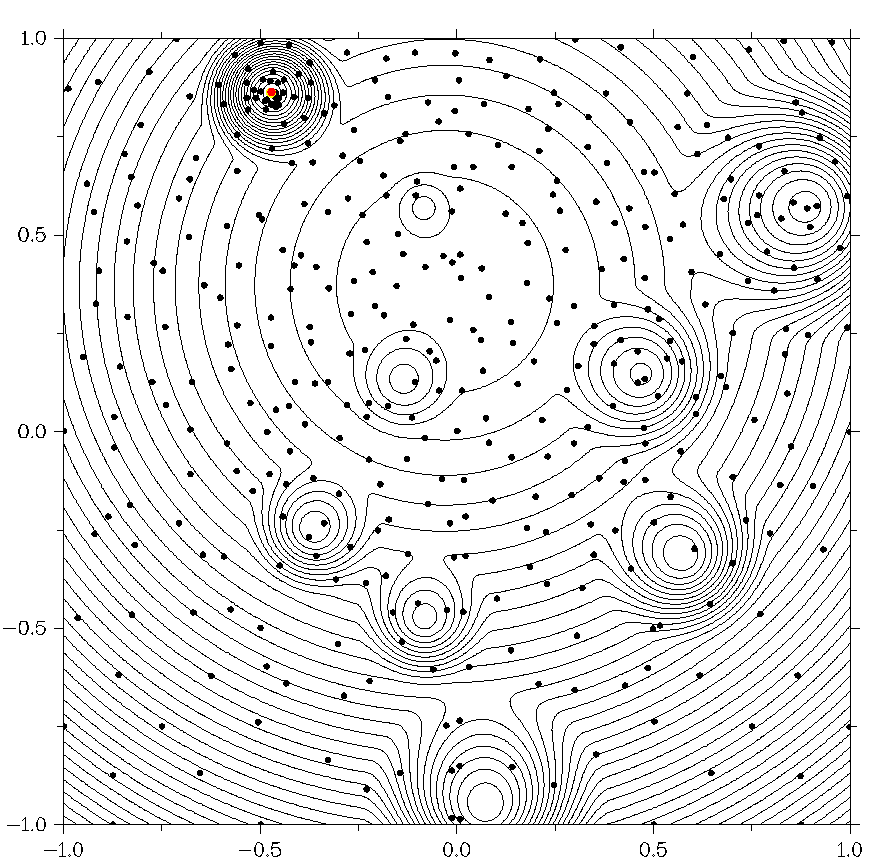
\includegraphics[width=1.0\linewidth]{GKLS-4.png} \\ (a)}
\end{minipage}
\hfill
\begin{minipage}{0.48\linewidth}
\center{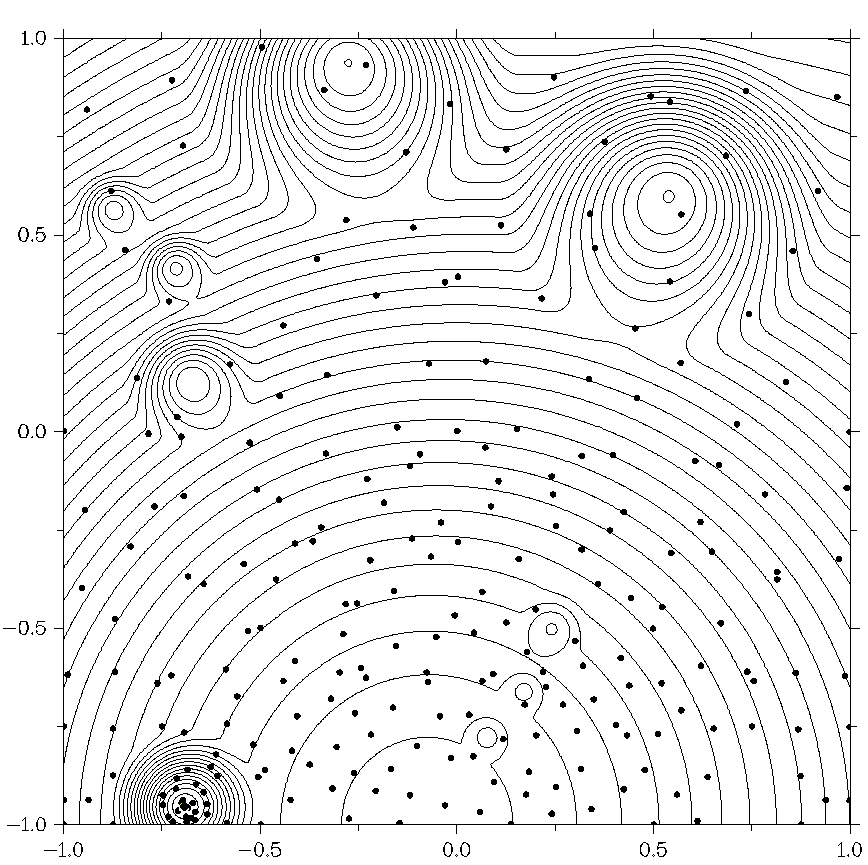
\includegraphics[width=1.0\linewidth]{GKLS-6.png} \\ (b)}
\end{minipage}
\caption{Solving a two-dimensional problem using the global search algorithm}
\label{example}
\end{figure}

В проведенных экспериментах генератор GKLS использовался как основа для построения mixed-integer problems. Правила, позволяющие генерировать тестовые задачи подобного вида, заключаются в следующем.

\begin{enumerate}
	\item С помощью генератора порождается непрерывная многоэкстремальная функция $\psi(y), \; y\in D, \; D = \left\{ a_j\leq y_j\leq b_j, 1\leq j \leq N \right\}$. Глобальный минимум данной функции достигается в известной точке $y'=(y'_1,...,y'_N)$ и равен $\psi'=\psi(y')=-1$.
	\item Генерируется convex mixed-integer function 
	\[
			\phi (y,u) = 2 \left[ \sum_{j=1}^N \left( \frac{y_j - y'_j}{b_j-a_j} \right)^2 + \sum_{j=1}^M \left( \frac{u_j - b_j}{b_j-a_j} \right)^2 \right],
	\]
	где 
	\begin{eqnarray*}
	& y\in D = \left\{ a_j\leq y_j\leq b_j, 1\leq j \leq N \right\} \subset R^N, \\
	& u\in U = \left\{ u_j \in  \left\{a_j, ..., b_j \right\}, 1\leq j \leq M \right\};
	\end{eqnarray*}
	т.е. данная функция имеет $N$ непрерывных и $M$ дискретных параметров и достигает минимального значения в точке $(y',b)$.
	\item Вычисляется коэффициент 
	\[
	C = 4 - \max_{y,u} \left\{ \phi(y,u) \right\}, \; y\in D, u \in U.
	\]
	Максимум выпуклой функции $\phi(y,u)$ достигается в одной из угловых точек области поиска, поэтому при размерности задачи порядка 10 его вычисление может быть выполнено методом перебора.
	\item Формируется многоэкстремальная mixed-integer function 
	\[
	\varphi(y,u) = \left(\psi(y) - \sum_{j=1}^M{u_j}\right)\left(C - \phi(y,u)\right).
	\]
	По построению $\varphi(y,u)$  будет принимать минимальное значение в точке $(y',b)$.
	
\end{enumerate}


In the problems generated in our experiments, there were 5 discrete and 4 continuous parameters 
	\begin{eqnarray*}
	& y\in D = \left\{ -1 \leq y_j\leq 1, 1\leq j \leq 4 \right\} \subset R^4, \\
	& u\in U = \left\{ u_j \in  \left\{-1, -1/3, 0, 1/3, 1 \right\}, 1\leq j \leq 5 \right\}.
	\end{eqnarray*}


Было сгенерировано и решено 100 9-и мерных mixed-integer problems данного типа. С целью имитации вычислительной трудоемкости, присущей прикладным задачам оптимизации, расчет функции во всех проводимых экспериментах был усложнен дополнительными вычислениями, не меняющими вид функции и расположение ее минимумов.
The accuracy of the search was equal to $10^{-2}$. Computational experiments were carried out on Lobachevsky supercomputer. The node of supercomputer included two Intel Sandy Bridge E5-2660 2.2 GHz CPUs and 64 Gb RAM. 

В Table \ref{tab:2} приведены результаты экспериментов, полученные для последовательной версии алгоритма PMGAL с использованием различных стратегий чередования локального и глобального поиска. Для локального поиска в формулах (\ref{lR}) использовался параметр $q=3$, для глобального -- $q=0$. В первом столбце таблицы отражена частота чередования указанных значений. Например, 1:1 соответствует чередованию локального и глобального поиска на каждой итерации, 1:2 соответствует одному шагу локального поиска и двум шагам глобального поиска, и т.д. Во втором столбце таблицы отражено среднее число итераций $K_{av}$ (тыс.), требуемое для решения задачи с заданной точностью.

\begin{table}
	\caption{Сравнение стратегий local tuning}
	\label{tab:2}
	\center
	\begin{tabular}{|c|c|}
		\hline		
		\textit{loc} : \textit{glob} & $K_{av}$   \\
		\hline 
		1 : 1 & 102.6\\
		1 : 2 & 89.2\\
		1 : 4 & 97.5\\
		1 : 8 & 127.1\\
		1 : 16 & 144.2\\
		\hline
	\end{tabular}
\end{table}	


Результаты экспериментов показывают, что наименьшее число итераций методу с локальной настройкой требуется при использовании стратегии чередования 1:2, т.е. один шаг локального уточнения чередуется с двумя шагами глобального поиска. Будем использовать эту стратегию и в дальнейших экспериментах.

\begin{table}
	\caption{Среднее время работы $T_{av}$ параллельного алгоритма с локальной настройкой}
	\label{tab:3}
	\center
	\begin{tabular}{|c|c|c|c|}
		\hline	
	\diaghead{\theadfont Diag Column} { $N_{p}$}{$N_{t}$} & 1 & 4 & 8\\
	
		\hline		
		2  & 199.0 & 65.4 & 61.0  \\
		5  & 91.2 & 28.0 &  26.1 \\
		17  & 37.2 & 10.8 & 7.5 \\
		65  & 29.3 & 8.7 & 5.4 \\
		\hline
	\end{tabular}
\end{table}	


Последняя серия экспериментов была выполнена для оценки ускорения параллельной версии алгоритма PMGAL. 
В Table \ref{tab:3} приведено среднее время решения $T_{av}$ (в секундах) в зависимости от задействованного числа процессов $N_{p}$ и потоков $N_{t}$ в каждом процессе. При проведении экспериментов было задействовано от 1 до 16 узлов кластера в зависимости от числа параллельных процессов. 
Ускорение, которое демонстрирует параллельный алгоритм, не является идеальным, но -- вполне приемлемое.   


\section{Conclusions}

В данной статье представлены результаты, связанные с разработкой параллельных алгоритмов глобальной оптимизации для решения многоэкстремальных задач, в которых часть параметров является непрерывными, а часть -- дискретными.
Рассматриваемые задачи могут включать в себя также невыпуклые ограничения, учет которых организован с использованием специальной индексной схемы. 
Для задач указанного класса предложен параллельный алгоритм их решения. Основной принцип организации параллельных вычислений в алгоритме основан на одновременном проведении нескольких испытаний в различных точках области поиска. 

В параллельном алгоритме глобальной оптимизации использована техника локальной настройки, основанная на предположении слабой многоэкстремальности задачи. Данное предположение является верным, в частности, на заключительной фазе поиска, когда уже выполнено одно или несколько испытаний в окрестности глобального решения, и осталось найденную оценку решения уточнить.

В последовательном варианте предложенный алгоритм не уступает методам аналогичного назначения, реализованным в Matlab Global Optimization Toolbox.
В параллельном варианте предложенный алгоритм демонстрирует приемлемую масштабируемость вплоть до ипользования десятков параллельных процессов. 


\begin{acknowledgments}
This work was supported by the Ministry of Science and Higher Education of the Russian Federation, project no. 0729-2020-0055, and by the Research and Education Mathematical Center, project no. 075-02-2020-1483/1.
\end{acknowledgments}


%
% The Bibliography
%

\begin{thebibliography}{99}

\bibitem{Burer}
S.~Burer and A.~N.~Letchford, \textit{Non-convex mixed-integer nonlinear programming: A survey}, Surveys in Operations Research and Management Science \textbf{17}, 97--106 (2012).

\bibitem{Boukouvala}
F.~Boukouvala, R.~Misener and C.~A.~Floudas, \textit{Global optimization advances in Mixed-Integer Nonlinear Programming, MINLP, and Constrained Derivative-Free Optimization, CDFO}, European J. Oper. Res. \textbf{252}, 701--727 (2016).

\bibitem{Belotti}
P.~Belotti, J.~Lee, L.~Liberti, F.~Margot and A.~W\"achter, \textit{Branching and bounds tightening techniques for non-convex MINLP}, Optim. Method. Softw. \textbf{24}(4-5), 597--634 (2009).

\bibitem{Vigerske}
S.~Vigerske and A.~Gleixner, \textit{SCIP: global optimization of mixed-integer nonlinear programs in a branch-and-cut framework}, Optim. Method. Softw. \textbf{33}(3), 563--593 (2018).

\bibitem{Deep}
K.~Deep, K.~P.~Singh, M.~L.~Kansal and C.~Mohan, \textit{A real coded genetic algorithm for solving integer and mixed integer optimization problems}, Appl. Math. Comput. \textbf{212}(2), 505--518 (2009).

\bibitem{Schluter}
M.~Schl\"uter, J.~A.~Egea and J.~R.~Banga, \textit{Extended ant colony optimization for non-convex mixed integer nonlinear programming}, Computers and Operations Research \textbf{36}(7), 2217--2229 (2009).

\bibitem{Evtushenko2009} 
Yu.~G.~Evtushenko, V.~U.~Malkova and A.~A.~Stanevichyus, \textit{Parallel global optimization of functions of several variables}, Computational Mathematics and Mathematical Physics \textbf{49}(2), 246--260 (2009).

\bibitem{Zilinskas2011}
R.~Paulavi\v{c}ius, J.~\v{Z}ilinskas and A.~Grothey, \textit{Parallel branch and bound for global optimization with combination of Lipschitz bounds}. Optimization Methods \& Software \textbf{26}(3), 487--498 (2011).

\bibitem{Zilinskas2014}
R.~Paulavi\v{c}ius and J.~\v{Z}ilinskas, \textit{Simplicial Global Optimization} (Springer Briefs in Optimization. Springer, 2014).

\bibitem{Sergeyev2017}
Y.~D.~Sergeyev and D.~E.~Kvasov, \textit{Deterministic Global Optimization. An Introduction to the Diagonal Approach}  (Springer Briefs in Optimization, Springer, 2017).


%\bibitem{Evtushenko2013} Y.~G.~Evtushenko and M.~A.~Posypkin, \textit{A deterministic approach to global box-constrained optimization}, Optim. Lett. \textbf{7}(4), 819--829 (2013).
	
\bibitem{Strongin2000}
R.~G.~Strongin and Y.~D.~Sergeyev, \textit{Global optimization with non-convex constraints. Sequential and parallel algorithms} (Kluwer Academic Publishers, Dordrecht, 2000, 2nd ed. 2013, 3rd ed. 2014).

\bibitem{Strongin2013}
R.~G.~Strongin, V.~P.~Gergel, V.~A.~Grishagin and K.~A.~Barkalov, \textit{Parallel computations for global optimization problems} (Moscow State University, Moscow, 2013) [In Russian].

\bibitem{Sergeyev2013}
Ya.~D.~Sergeyev, R.~G.~Strongin and D.~Lera, \textit{Introduction to Global Optimization Exploiting Space-Filling Curves} (Springer Briefs in Optimization, Springer, 2013).


\bibitem{Strongin2020}
R.~Strongin, K.~Barkalov and S.~Bevzuk, \textit{Global optimization method with dual Lipschitz constant estimates for problems with non-convex constraints}, Soft Computing \textbf{24}(16), 11853--11865 (2020).

\bibitem{Gergel2020}
V.~Gergel, E.~Kozinov and K.~ Barkalov, \textit{Computationally efficient approach for solving lexicographic multicriteria optimization problems}, Optim. Lett. (2020). DOI: 10.1007/s11590-020-01668-y 

\bibitem{Sergeyev2003}
Y.~D.~Sergeyev, P.~Pugliese and D.~Famularo, \textit{Index information algorithm with local tuning for solving multidimensional global optimization problems with multiextremal constraints}, Math. Program. \textbf{96}(3), 489--512 (2003).
2003.

\bibitem{Sergeyev2007}
Y.~D.~Sergeyev, D.~E.~Kvasov and F.~M.~H.~Khalaf, \textit{A one-dimensional local tuning algorithm for solving GO problems with partially defined constraints} Optimization Letters \textbf{1}(1), 85--99 (2007).

\bibitem{Sergeyev2020}
D.~E.~Kvasov, M.~S.~Mukhametzhanov, M.~C.~Nasso and Y.~D.~Sergeyev, \textit{On acceleration of derivative-free univariate Lipschitz global optimization methods}, Lecture Notes in Computer Science \textbf{11974}, 413--421 (2020).

\bibitem{Barkalov2010}
K.~Barkalov, V.~Ryabov, S.~Sidorov, \textit{Parallel scalable algorithms with mixed local-global strategy for global optimization problems}, Lecture Notes in Computer Science \textbf{6083}, 232–240 (2010).
 
\bibitem{Strongin2018}
R.~G.~Strongin, V.~P.~Gergel, K.~A.~Barkalov and A.~V.~Sysoyev, \textit{Generalized parallel computational schemes for time-consuming global optimization}, Lobachevskii Journal of Mathematics \textbf{39}(4), 576--586 (2018.)

\bibitem{Barkalov2020}
R.~G.~Strongin, V.~P.~Gergel and K.~A.~Barkalov, \textit{Adaptive global optimization based on a block-recursive dimensionality reduction scheme}, Automation and Remote Control \textbf{81}(8), 1475--1485 (2020).

\bibitem{Floudas}
C.~A.~Floudas and M.~P.~Pardalos,  \textit{Handbook of Test Problems in Local and Global Optimization}. (Springer, 1999).  %; DOI: 10.1007/978-1-4757-3040-1

\bibitem{Gaviano}
M.~Gaviano, D.~Lera, D.~E.~Kvasov and Ya.~D.~Sergeyev, \textit{Software for generation of classes of test functions with known local and global minima for global optimization}, ACM Trans. Math. Softw. \textbf{29}, 469--480 (2003).


%\bibitem{Floudas}
%C.~A.~Floudas and M.~P.~Pardalos, \textit{Recent advances in global optimization} (Princeton University Press, 2016).
%
%\bibitem{Locatelli}
%M.~Locatelli and F.~Schoen, \textit{Global optimization: theory, algorithms and applications} (SIAM, 2013).
%
%
%\bibitem{Pardalos}
%P.~M.~Pardalos, A.~A.~Zhigljavsky and J.~\v{Z}ilinskas \textit{Advances in stochastic and deterministic global optimization} (Springer, 2016).
%
%
%\bibitem{Ciegis}
%R.~\v{C}iegis, D.~Henty, B.~K\r{a}gstr\"om and J.~\v{Z}ilinskas, \textit{Parallel scientific computing and optimization: advances and applications}  (Springer, 2009). 
%
%\bibitem{Luque}
%G.~Luque and E.~Alba, \textit{Parallel genetic algorithms. Theory and real world applications} (Springer-Verlag, Berlin, 2011).
%
%\bibitem{Strongin3}
%R.~G.~Strongin, \textit{Numerical Methods in Multiextremal Problems (Information-Statistical Algorithms)} (Nauka, Moscow, 1978) [In Russian].
%
%\bibitem{Strongin4}
%R.~G.~Strongin and Y.~D.~Sergeyev, \textit{Global multidimensional optimization on parallel computer}, Parallel Computing \textbf{18} (11), 1259--1273 (1992).
%
%\bibitem{Sergeyev4}
%Y.~D.~Sergeyev and V.~A.~Grishagin, \textit{Parallel asynchronous global search and the nested optimization scheme}, J. Comput. Anal. Appl., \textbf{3} (2), 123--145 (2001).
%
%\bibitem{Gergel1}
%V.~P.~Gergel and S.~V.~Sidorov, \textit{A Two-Level Parallel Global Search Algorithm for Solution of Computationally Intensive Multiextremal Optimization Problems}, Lecture Notes in Computer Science \textbf{9251}, 505--515 (2015).
%
%\bibitem{Gergel2}
%V.~Gergel, \textit{An Unified Approach to Use of Coprocessors of Various Types for Solving Global Optimization Problems}, in Proceedings of the Second International Conference on Mathematics and Computers in Sciences and in Industry (MCSI), Sliema, 13--18 (2015).
%
%\bibitem{Barkalov}
%K.~Barkalov, V.~Gergel and I.~Lebedev, \textit{Solving global optimization problems on GPU cluster}, AIP Conference Proceedings \textbf{1738}, 400006 (2016).
%
%\bibitem{Gergel3}
%V.~Gergel and E.~Kozinov, \textit{Efficient methods of multicriterial optimization based on the intensive use of search information}, Springer Proceedings in Mathematics and Statistics \textbf{197}, 27--45 (2017). 
%
%\bibitem{Gergel4}
%V.~Gergel and E.~Kozinov, \textit{Parallel computing for time-consuming multicriterial optimization problems}, Lecture Notes in Computer Science \textbf{10421}, 446--458 (2017).
%
%\bibitem{Gergel5}
%V.~Gergel, V.~Grishagin and A.~Gergel, \textit{Adaptive nested optimization scheme for multidimensional global search}, J. Glob. Optim.  \textbf{66} (1), 35--51 (2016).
%
%\bibitem{Lera}
%D.~Lera, Y.~D.~Sergeyev, \textit{Lipschitz and Holder global optimization using space-filling curves},  Appl. Numer. Math. \textbf{60} (1-2), 115--129 (2010).
%
%\bibitem{Grishagin1}
%V~A.~Grishagin. \textit{On convergence conditions for a class of global search algorithms}, in Proceedings of the 3-rd All-Union seminar ``Numerical methods of nonlinear programming'', Kharkov, 82--84 (1979) [In Russian].
%
%\bibitem{Grishagin2}
%V.~A.~Grishagin, Y.~D.~Sergeyev and R.~G.~Strongin, \textit{Parallel characteristic algorithms for solving problems of global optimization}, J. Glob. Optim. \textbf{10} (2), 185--206 (1997).
%
%\bibitem{Strongin5}
%R.~G.~Strongin, \textit{Algorithms for Multi-extremal Mathematical Programming Problems Employing the Set of Joint Space-filling Curves}, J. Glob. Optim. \textbf{2} (4), 357--378 (1992).
%
%\bibitem{Sysoyev}
%A.~Sysoyev, K.~Barkalov, V.~Sovrasov, I.~Lebedev and V.~Gergel, \textit{Globalizer -- A parallel software system for solving global optimization problems}, Lecture Notes in Computer Science \textbf{10421}, 492--499 (2017). 
%
%\bibitem{Sergeyev7}
%Y.~D.~Sergeyev and V.~A.~Grishagin, \textit{Parallel Asynchronous Global Search and the Nested Optimization Scheme}, J. Comput. Anal. Appl. \textbf{3} (2), 123--145 (2001).
%
%\bibitem{Modorskii}
%V.~Y.~Modorskii, D.~F.~Gaynutdinova, V.~P.~Gergel and K.~A.~Barkalov, \textit{Optimization in design of scientific products for purposes of cavitation problems}, AIP Conference Proceedings \textbf{1738}, 400013 (2016).
%
%\bibitem{Gergel6}
%V.~P.~Gergel, M.~I.~Kuzmin, N.~A.~Solovyov and V.~A.~Grishagin, \textit{Recognition of surface defects of cold-rolling sheets based on method of localities}, International Review of Automatic Control \textbf{8} (1), 51--55 (2015).


\end{thebibliography}
\end{document}
